% Compilar com XeLaTeX (no Overleaf: Menu > Compiler > XeLaTeX).
\documentclass[12pt,a4paper]{article}

\usepackage{fontspec}
\IfFontExistsTF{Arial}{\setmainfont{Arial}}{%
  \IfFontExistsTF{Liberation Sans}{\setmainfont{Liberation Sans}}{\setmainfont{TeX Gyre Heros}}}
\usepackage[provide=*,brazilian]{babel}
\usepackage[a4paper,top=3cm,left=3cm,bottom=2cm,right=2cm,headheight=15pt,headsep=0.6cm]{geometry}
\usepackage{setspace}
\usepackage{indentfirst}
\usepackage{graphicx}
\usepackage{booktabs}
\usepackage{array}
\usepackage{titlesec}
\usepackage{fancyhdr}
\usepackage[font=footnotesize,labelsep=endash,justification=centering,skip=4pt]{caption}
\usepackage{xurl}
\usepackage[hidelinks]{hyperref}
\urlstyle{same}

\graphicspath{{figuras/}}
\onehalfspacing
\setlength{\emergencystretch}{1.5em}
\setlength{\parindent}{1.25cm}
\setlength{\parskip}{0pt}
\setlength{\footnotesep}{10pt}
\renewcommand{\footnotesize}{\fontsize{10pt}{12pt}\selectfont}

\pagestyle{fancy}
\fancyhf{}
\fancyhead[R]{\fontsize{10pt}{12pt}\selectfont\thepage}
\renewcommand{\headrulewidth}{0pt}

\titleformat{\section}{\normalfont\bfseries}{\thesection}{0.5em}{\MakeUppercase}
\titlespacing*{\section}{0pt}{18pt}{12pt}
\titleformat{\subsection}{\normalfont\bfseries}{\thesubsection}{0.5em}{}
\titlespacing*{\subsection}{0pt}{12pt}{6pt}

\newcommand{\repo}{\url{https://github.com/Marivan-Olivares/Ecotriagem}}
\newcommand{\fonte}[1]{\par\vspace{2pt}{\footnotesize\raggedright #1\par}}
\newcommand{\secaosemnumero}[1]{\begin{center}\textbf{\MakeUppercase{#1}}\end{center}}

\begin{document}
\thispagestyle{fancy}

\begin{center}
\textbf{ECOTRIAGEM}
\end{center}

\vspace{12pt}
\noindent Integrantes: Marivan Olivares; Humberto Torres; Vinicius

\vspace{6pt}
\begin{singlespace}
\secaosemnumero{Resumo}
O descarte incorreto de resíduos contamina materiais recicláveis e reduz a eficiência da coleta seletiva. Este trabalho apresenta o EcoTriagem, aplicação que integra visão computacional, processamento de linguagem natural (PLN), aprendizado de máquina e tomada de decisão para identificar o material de um resíduo por foto e orientar o descarte a partir de perguntas em português. A imagem é descrita por uma MobileNetV2 pré-treinada e classificada por uma máquina de vetores de suporte (SVM) com calibração isotônica, e o rótulo é lido por reconhecimento óptico de caracteres (OCR). As perguntas são classificadas em nove intenções por TF-IDF e SVM linear, e um agente baseado em objetivos combina as evidências por regras sensíveis à confiança, acionando uma busca A* até o ponto de coleta mais próximo. No TrashNet, o classificador atingiu 88,9\% de acurácia e 95,6\% de acerto nas decisões automáticas de alta confiança; o reconhecimento de intenções obteve F1-macro de 0,852 em teste redigido manualmente; e, em 379 cenários ponta a ponta, o sistema acertou 91,2\% dos materiais quando respondeu, abstendo-se em 4,5\% dos casos.

\end{singlespace}

\section{Introdução}
A Política Nacional de Resíduos Sólidos (PNRS) prevê a coleta seletiva e a logística reversa, e a Resolução CONAMA n.º 275/2001 padronizou as cores dos coletores de recicláveis. Na prática, porém, o cidadão muitas vezes não sabe de que material é um objeto, em qual coletor descartá-lo nem onde entregá-lo. A separação incorreta contamina o material reciclável.

Classificadores de imagens de resíduos já foram propostos, mas costumam ser avaliados isoladamente, apenas pela acurácia, sem considerar como a confiança da previsão deve orientar a decisão nem como o usuário formula sua dúvida. O objetivo deste trabalho é projetar, implementar e avaliar uma aplicação em que visão computacional e PLN atuam no mesmo fluxo: o usuário envia uma foto, faz perguntas em português e um agente combina as evidências para responder de forma contextualizada.

As contribuições são: um sistema integrado e reprodutível em CPU; um critério de seleção de modelos baseado na qualidade da confiança; a identificação de fotos duplicadas com rótulos conflitantes no TrashNet; e um conjunto autoral de intenções em português.

\section{Fundamentação teórica e trabalhos relacionados}
Um agente baseado em objetivos mantém um estado interno e escolhe ações que o aproximam de um objetivo, e regras com encadeamento para frente tornam a decisão explicável. O A* expande nós em ordem de f(n) = g(n) + h(n) e é ótimo quando a heurística h é admissível.

Na visão computacional, a MobileNetV2 é uma rede convolucional leve cujas características pré-treinadas se transferem bem para outras tarefas. Como SVMs não produzem probabilidades, estas podem ser obtidas por calibração isotônica. No PLN, TF-IDF com classificadores lineares é uma linha de base forte para textos curtos.

No TrashNet, Siqueira comparou quatro redes convolucionais, entre elas a MobileNetV2, e obteve 91,97\% de acurácia com uma ResNet34. Esses trabalhos tratam a classificação isoladamente, enquanto o presente estudo a integra ao PLN e à decisão.

\section{Metodologia}
\subsection{Arquitetura do sistema}
A Figura~\ref{fig:arq} resume o fluxo. A imagem é padronizada com OpenCV, descrita pela MobileNetV2 e classificada; em paralelo, o OCR lê o rótulo. A pergunta é normalizada, classificada em uma intenção e analisada por um extrator de entidades. O agente guarda em seu estado a última imagem e o bairro do usuário, o que permite diálogos encadeados. O motor de regras funde as evidências, consulta a base de conhecimento e, se necessário, executa a busca A*.

\begin{figure}[!htb]
\centering
\caption{Arquitetura do EcoTriagem}\label{fig:arq}
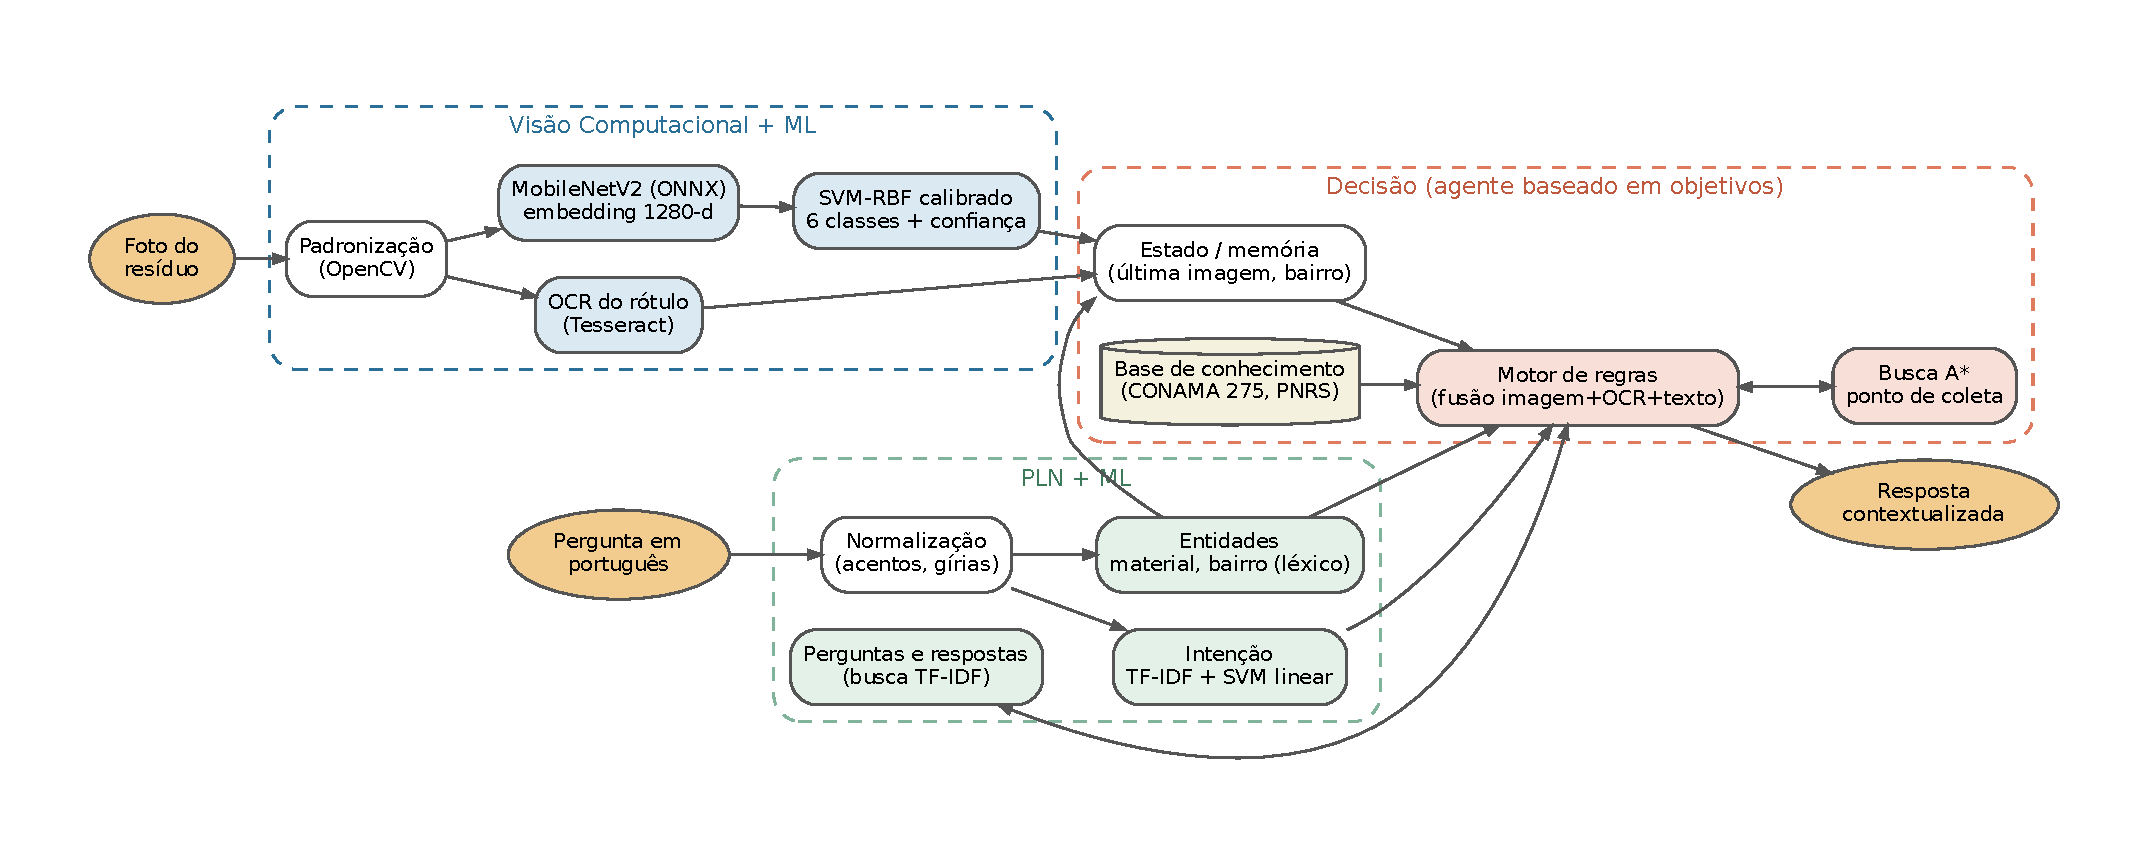
\includegraphics[width=\textwidth]{arquitetura.pdf}
\end{figure}

\subsection{Dados}
Utilizou-se o TrashNet, com 2.527 fotos em seis classes. Três pares de fotos idênticas com rótulos diferentes foram removidos, e as 2.521 imagens restantes foram divididas de forma estratificada em treino, validação e teste (70/15/15\%), com o F1-macro como métrica principal devido ao desbalanceamento.

A equipe construiu um conjunto de nove intenções em português, com 1.170 frases de treino geradas a partir de 190 modelos de frase e 132 frases de teste escritas à mão. As regras seguem a PNRS e a CONAMA 275/2001, e o mapa simula 32 bairros de Maceió e dez pontos de coleta fictícios.

\subsection{Visão computacional e aprendizado de máquina}
Adotou-se aprendizado supervisionado. A MobileNetV2 pré-treinada foi usada como extratora congelada de características e comparada a um vetor clássico de cor, textura e forma, em sete combinações de classificadores. Os hiperparâmetros foram ajustados por validação cruzada de cinco dobras, apenas no treino.

A seleção exigiu, além do maior F1-macro na validação, confiança calibrada e informativa, porque o modelo de maior F1, a SVM com calibração de Platt, gerava confianças que mal distinguiam acertos de erros. Os limiares de decisão, definidos na validação, foram 0,84 e 0,60. O OCR usa o Tesseract 5, e termos do rótulo como “PET” e “alumínio” são mapeados para materiais.

\subsection{Processamento de linguagem natural}
O texto é normalizado e representado por TF-IDF de palavras e de caracteres; Naive Bayes, regressão logística e SVM linear foram comparados por validação cruzada. Intenções com probabilidade inferior a 0,35 levam o sistema a pedir reformulação, e material e bairro são extraídos por um léxico de 160 termos.

\subsection{Agente, regras e busca}
O motor de regras (22 regras) resolve o material nesta ordem: um material citado no texto prevalece; com confiança ≥ 0,84, aceita-se a imagem; abaixo disso, usa-se o material lido pelo OCR, se houver (fusão); entre 0,60 e 0,84, aceita-se a imagem e pede-se confirmação; abaixo de 0,60, o sistema pede outra foto. Para localizar o ponto de coleta, os estados são bairros, o objetivo é qualquer bairro com ponto que aceite o material, e a heurística é a menor distância em linha reta até um objetivo. Essa heurística é admissível e consistente, o que garante a otimalidade do A*.

\subsection{Ambiente, experimentos e métricas}
A implementação usou Python 3.13, scikit-learn, OpenCV, Tesseract 5 e Streamlit, em CPU sem GPU, e o teste foi usado uma única vez por modelo. Os experimentos avaliaram modelos, calibração, robustez, OCR com fusão, busca e o sistema ponta a ponta, com acurácia, F1-macro, ECE, AUROC, nós expandidos, custo da rota e latência.

\section{Resultados e discussão}
\subsection{Classificação visual e confiança}
Os embeddings da MobileNetV2 superaram as características clássicas em até 10,8 pontos percentuais (Tabela~\ref{tab:visao}). O modelo selecionado obteve 88,9\% de acurácia no teste. A classe rejeito foi a mais difícil, e os erros mais frequentes associaram-se a reflexos.

\begin{table}[!htb]
\centering
\caption{Classificação visual (validação: 377 imagens; teste: 379 imagens)}\label{tab:visao}
{\footnotesize\singlespacing
\begin{tabular}{lcccc}
\toprule
\textbf{Modelo} & \textbf{F1-macro} & \textbf{AUROC} & \textbf{Acurácia} & \textbf{F1-macro} \\
 & \textbf{(val.)} & \textbf{(val.)} & \textbf{(teste)} & \textbf{(teste)} \\
\midrule
Clássico + Random Forest & 0,758 & 0,83 & 0,792 & 0,794 \\
CNN + SVM (Platt) & 0,870 & 0,62 & 0,884 & 0,867 \\
CNN + SVM (isotônica)* & 0,852 & 0,82 & 0,889 & 0,858 \\
\bottomrule
\end{tabular}\par}
\fonte{Fonte: Elaborada pelos autores (2026).\\Nota: * modelo selecionado (maior F1 com AUROC ≥ 0,75 e ECE ≤ 0,05 na validação).}
\end{table}

O ECE no teste foi de 0,044: 72,6\% das imagens tiveram confiança ≥ 0,84, com 95,6\% de acerto, e os 4,5\% abaixo de 0,60 acertariam só 41,2\%, justamente os casos em que o sistema pede nova foto. Sob perturbações, o modelo perdeu no máximo 4,2 pontos percentuais, exceto na oclusão de 25\%, em que caiu para 0,594 (Figura~\ref{fig:robustez}). Com etiquetas sintéticas, a fusão com o OCR elevou as decisões corretas de 82,7\% para 88,3\%.

\begin{figure}[!htb]
\centering
\caption{Acurácia no teste sob perturbações das imagens}\label{fig:robustez}
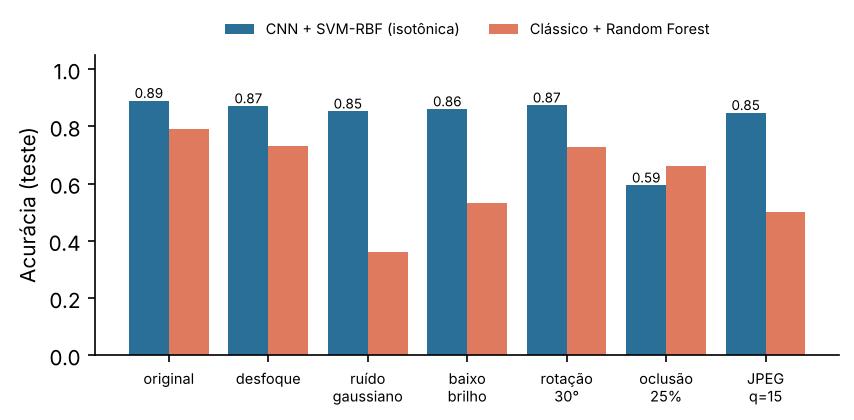
\includegraphics[width=0.75\textwidth]{visao_robustez.png}
\end{figure}

\subsection{Reconhecimento de intenções}
Na validação cruzada sobre frases geradas, o F1-macro chegou a 0,992, mas no teste manual a SVM linear obteve 0,852, o que mostra que avaliar só com frases geradas é otimista. Os n-gramas de caracteres acrescentaram de 9 a 12 pontos, e o extrator de entidades obteve F1 de 0,976 para material e 1,00 para bairro.

\subsection{Busca e avaliação ponta a ponta}
O A* encontrou sempre o caminho ótimo, expandindo 44\% menos nós que a busca de custo uniforme; a busca gulosa gerou rotas até 83\% mais longas.

Nos 379 cenários ponta a ponta, o sistema se absteve em 4,5\% dos casos e, quando respondeu, acertou o material em 91,2\%, com latência mediana de 249 ms por imagem. Em um exemplo real, para a foto de um vidro seguida de “isso é reciclável?” e “onde fica o ponto de coleta mais próximo do Benedito Bentes?”, o sistema indicou o coletor verde e um ecoponto fictício a 5,9 km, com rota obtida pelo A*.

Como limitações, o TrashNet tem fundo e iluminação controlados, o OCR foi avaliado com etiquetas sintéticas e os pontos de coleta são simulados.

\section{Conclusão e trabalhos futuros}
Os objetivos foram atingidos: o EcoTriagem integra visão computacional, PLN, aprendizado de máquina, regras e busca A* em um fluxo único executável em CPU, com 88,9\% de acurácia visual e 91,2\% de acerto ponta a ponta quando responde. O trabalho mostra ainda que a seleção de modelos para decisão deve considerar a qualidade da confiança. Como trabalhos futuros, propõem-se o ajuste fino com fotos reais, novas classes de resíduos e a integração com a base oficial de ecopontos.

\vspace{12pt}
\secaosemnumero{Contribuição dos autores}
\textbf{Marivan Olivares:} preparação do TrashNet e remoção de duplicatas; módulo de visão computacional (MobileNetV2, classificadores e calibração) e OCR; experimentos de classificação, calibração, robustez e fusão.

\textbf{Humberto Torres:} construção do conjunto de intenções em português; módulo de PLN (normalização, classificador de intenções, extrator de entidades e base de perguntas e respostas) e sua avaliação.

\textbf{Vinicius:} base de conhecimento, motor de regras, mapa e busca A* com a comparação de algoritmos; integração em Streamlit, avaliação ponta a ponta e repositório no GitHub. Todos participaram da definição da arquitetura e da redação do artigo.

\vspace{12pt}
\secaosemnumero{Referências}
\begin{singlespace}
\setlength{\parindent}{0pt}
\setlength{\parskip}{12pt}
\raggedright

BRASIL. Lei n.º 12.305, de 2 de agosto de 2010. Institui a Política Nacional de Resíduos Sólidos. \textbf{Diário Oficial da União}: seção 1, Brasília, DF, 3 ago. 2010.

CASELI, H. M.; NUNES, M. G. V. (org.). \textbf{Processamento de linguagem natural}: conceitos, técnicas e aplicações em português. São Carlos: BPLN, 2023. Disponível em: \url{https://brasileiraspln.com/livro-pln/1a-edicao/}. Acesso em: 18 nov. 2026.

CONSELHO NACIONAL DO MEIO AMBIENTE (Brasil). Resolução n.º 275, de 25 de abril de 2001. Estabelece o código de cores para os diferentes tipos de resíduos. \textbf{Diário Oficial da União}: seção 1, Brasília, DF, 19 jun. 2001.

FACELI, K. \textit{et al}. \textbf{Inteligência artificial}: uma abordagem de aprendizado de máquina. 2. ed. Rio de Janeiro: LTC, 2021.

RUSSELL, S. J.; NORVIG, P. \textbf{Inteligência artificial}: uma abordagem moderna. 4. ed. Rio de Janeiro: LTC, 2022.

SIQUEIRA, L. P. \textbf{Identificação e classificação de lixo doméstico através de rede neural convolucional}: revisão e pesquisa de mercado. 2021. Trabalho de Conclusão de Curso (Graduação em Engenharia Química) – Escola de Engenharia, Universidade Federal do Rio Grande do Sul, Porto Alegre, 2021. Disponível em: \url{http://hdl.handle.net/10183/235795}. Acesso em: 18 nov. 2026.
\end{singlespace}

\end{document}
